\chapter{السطوح الفاصلة والمواد الفعالة سطحيًا والغروانيات}\label{ch:b3:colloids}

المايونيز زيت مشتت في صورة قُطيرات قطرها بضعة ميكرومترات في قليل من
الماء والخل، تُبقيها متباعدة الليسيثينات وبروتينات صفار البيض. فإذا خُفق
بسرعة مفرطة في البداية، أو صُبّ الزيت بسرعة كبيرة، انفصل إلى طبقة
زيتية وأخرى مائية: إذ تندمج القطيرات، وتزول الطاقة التي كانت تُبقيها
متباعدة. والحليب والضباب والحبر والطلاء والدم وماء النهر الموحل
من الصنف نفسه من المادة: جسيمات أو قطيرات أكبر بكثير من الجزيئات 
وأصغر بكثير من أي شيء تراه العين، وكثيرة إلى حد أن معظم جزيئاتها
قريبة من سطح فاصل. ويعالج هذا الفصل طاقة السطوح الفاصلة، 
والجزيئات التي تخفضها، والغروانيات التي تتيحها السطوح الفاصلة، وما
يُبقي الغروانيات مشتتة أو يجعلها تتخثر.

\begin{recall}
سمّى مجلد السنة الأولى محبًّا للوسطين جزيئًا له رأس محب للماء 
وذيل كاره للماء، ووصف تآثرات لندن والسماحية
النسبية للمذيبات؛ وصادف جزء الصف الحادي عشر من المجلد الأول المذيلات
في الصابون. وعرّف مجلد السنة الثانية الجهد الكيميائي والشدة الأيونية 
والنشاطية. وعالج \cref{ch:b3:surfaces-catalysis} \omterm{def:b3:surfaces-catalysis:adsorption}{الامتزاز} على الصلبة،
و\cref{ch:b3:electrode-kinetics} \omterm{def:b3:electrode-kinetics:double-layer}{الطبقة الكهربائية المزدوجة} \omterm{def:b3:electrode-kinetics:double-layer}{وطول ديباي}
الخاص بها. ومن الفيزياء: الحركة البراونية، والضغط داخل سطح
منحنٍ.
\end{recall}

\begin{omfigure}
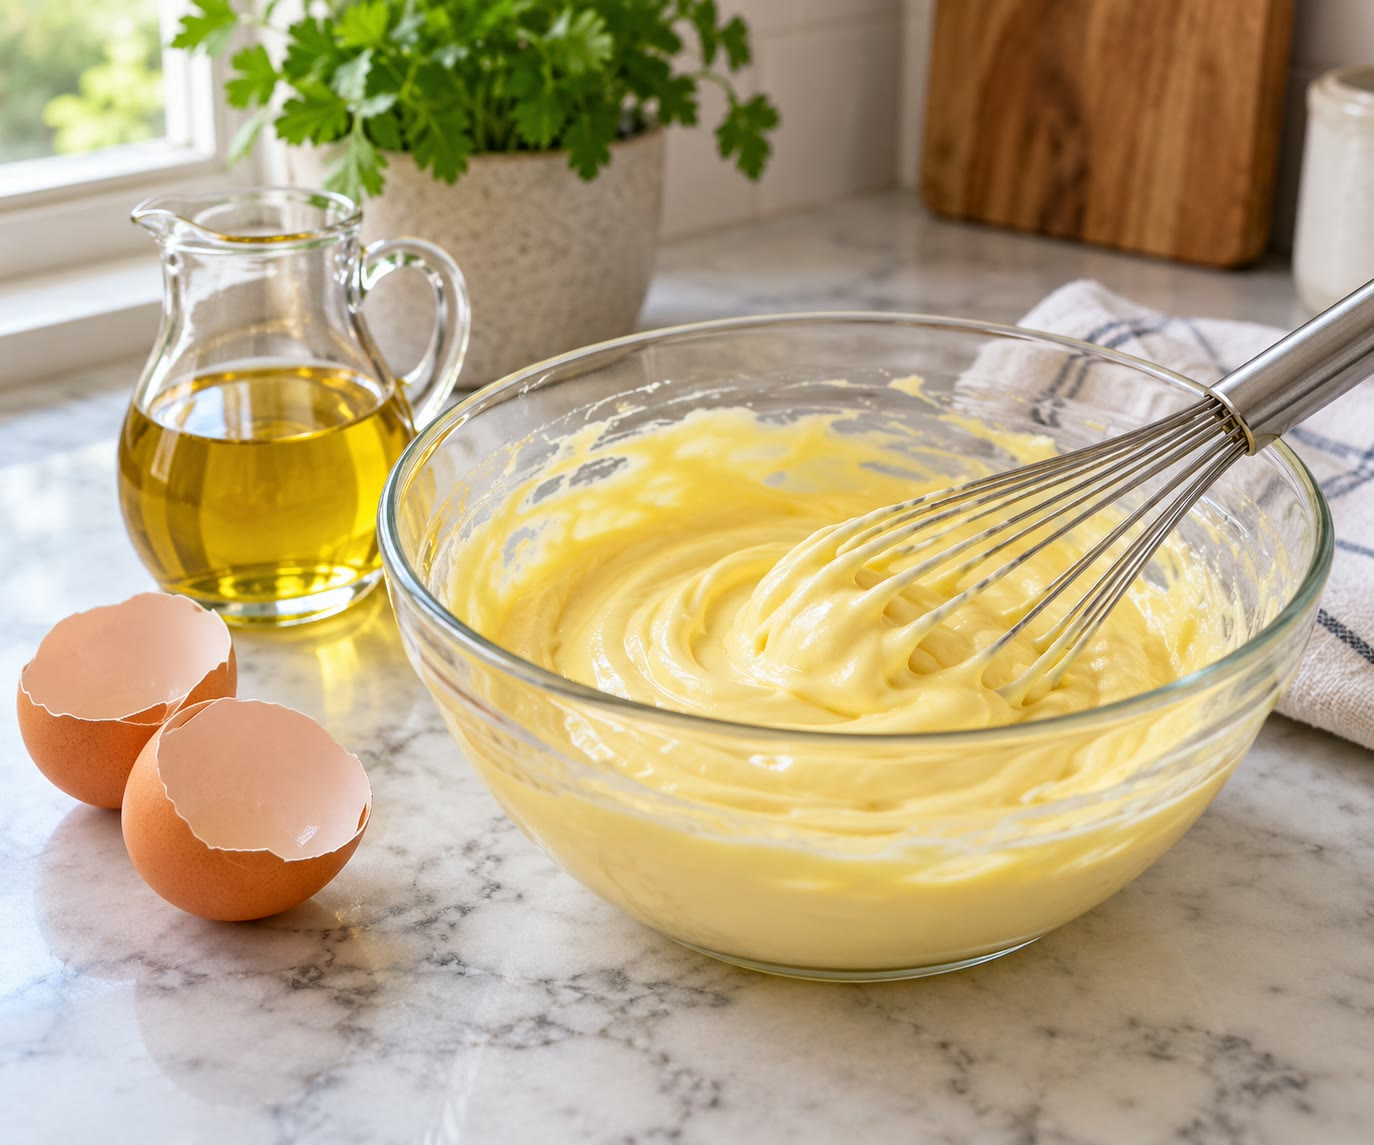
\includegraphics[width=0.6\linewidth]{images/book4/ai/b3-17-mayonnaise.jpg}

{\small خفق المايونيز: \omterm{def:b3:colloids:colloid}{مستحلب} من قطيرات الزيت في الماء،
تثبّته المواد الفعالة سطحيًا في صفار البيض.}
\end{omfigure}

\section{السطوح الفاصلة والتوتر السطحي}

يُجذب الجزيء في كتلة السائل بالتساوي في كل الاتجاهات؛ أما عند
السطح فيفقد بعض جيرانه. فإنشاء سطح يكلّف طاقة.

\begin{definition}[التوتر السطحي]\label{def:b3:colloids:surface-tension}
\emph{التوتر السطحي}\index{توتر سطحي} $\gamma$ لسائل هو طاقة جيبس
اللازمة لإنشاء وحدة مساحة من سطحه عند درجة حرارة وضغط وتركيب
ثابتة: $\gamma = (\partial G/\partial A)_{T,p,n}$، بوحدة \unit{J.m^{-2}} $=$ \unit{N.m^{-1}}. ومن أجل
سطح فاصل بين طورين يسمى التوتر البيني.
\end{definition}

للماء، المتماسك بالروابط الهيدروجينية، \omterm{def:b3:colloids:surface-tension}{توتر سطحي} مرتفع: \qty{72.0}{mN/m}
عند \qty{25}{\celsius}. وللألكانات نحو 20، وللزئبق نحو 480.

\begin{proposition}[ضغط لابلاس]\label{prop:b3:colloids:laplace}
يزيد الضغط داخل قطرة أو فقاعة كروية نصف قطرها $r$ على
الضغط في الخارج بمقدار
\[
  \Delta p = \frac{2\gamma}{r} .
\]
\end{proposition}

\begin{proof}
لنزد نصف القطر بمقدار $\dd r$ عند التوازن: فالشغل الذي يبذله فرق
الضغط، $\Delta p\,4\pi r^2\dd r$، يساوي زيادة طاقة جيبس السطحية، $\gamma\,8\pi r\,\dd r$.
\end{proof}

\begin{definition}[زاوية التماس، التبلل]\label{def:b3:colloids:wetting}
\emph{زاوية التماس}\index{زاوية التماس} $\theta$ لقطرة على صلب هي الزاوية،
المقيسة عبر السائل، بين سطح الصلب وسطح السائل
عند الخط الذي يلتقي فيه الصلب والسائل والبخار. ويقال إن السائل \emph{يبلّل}\index{تبلل}
الصلب حين $\theta < 90^\circ$، وإنه ينتشر عليه كليًا حين $\theta = 0$.
\end{definition}

\begin{theorem}[معادلة يونغ]\label{thm:b3:colloids:young}
عند التوازن تحقق التوترات البينية الثلاثة \omterm{def:b3:colloids:wetting}{وزاوية التماس} العلاقة
\[
  \gamma_{\mathrm{SV}} = \gamma_{\mathrm{SL}} + \gamma_{\mathrm{LV}}\cos\theta .
\]
وهذه هي \emph{معادلة يونغ}\index{معادلة يونغ}.
\end{theorem}

\begin{proof}
لنحرّك خط التماس نحو الخارج بمقدار $\dd x$ (لكل وحدة طول من الخط): فيحل محل سطح
فاصل صلب--بخار مساحته $\dd x$ سطح فاصل صلب--سائل، ويكبر السطح الفاصل
سائل--بخار بمقدار $\dd x\cos\theta$. فتتغير طاقة جيبس بمقدار
$(\gamma_{\mathrm{SL}} - \gamma_{\mathrm{SV}} + \gamma_{\mathrm{LV}}\cos\theta)\dd x$، وهو معدوم عند التوازن.
\end{proof}

\begin{omfigure}
\begin{tikzpicture}[font=\small, >=Stealth]
  \fill[black!12] (-3.6,-0.5) rectangle (3.6,0);
  \draw[thick] (-3.6,0) -- (3.6,0);
  \node[anchor=north] at (2.6,-0.05) {\foreignlanguage{arabic}{الصلب}};
  \fill[omWater!60] (-2.0,0) arc[start angle=160, end angle=20, radius=2.13] -- cycle;
  \draw[thick, omDef] (-2.0,0) arc[start angle=160, end angle=20, radius=2.13];
  % circle centre 0.73 below the solid: a cap smaller than a hemisphere, contact angle 90 - 20 = 70 deg;
  % at the right contact point the liquid surface leaves at 110 deg (up and to the left)
  \draw[->, thick, omThm] (2.0,0) -- ++(110:1.3) node[anchor=south] {$\gamma_{\mathrm{LV}}$};
  \draw[->, thick] (2.0,0) -- (3.3,0) node[anchor=south] {$\gamma_{\mathrm{SV}}$};
  \draw[->, thick] (2.0,0) -- (0.7,0) node[anchor=north, yshift=-1pt] {$\gamma_{\mathrm{SL}}$};
  \draw (1.45,0) arc[start angle=180, end angle=110, radius=0.55];
  \node at (1.33,0.42) {$\theta$};
  \node at (0,0.6) {\foreignlanguage{arabic}{السائل}};
  \node at (-2.8,1.4) {\foreignlanguage{arabic}{البخار}};
\end{tikzpicture}

{\small قطرة جاثمة والتوترات الثلاثة التي تشد خط تماسها:
توازن مركّباتها على امتداد الصلب يعطي \omterm{thm:b3:colloids:young}{معادلة يونغ}؛ وهنا $\theta
\approx 70^\circ$، أي سائل \omterm{def:b3:colloids:wetting}{يبلّل} جزئيًا.}
\end{omfigure}

\begin{theorem}[معادلة كلفن]\label{thm:b3:colloids:kelvin}
يزيد ضغط بخار قطرة كروية نصف قطرها $r$ على ضغط بخار السائل
المستوي، $p^*$:
\[
  \ln\frac{p}{p^*} = \frac{2\gamma V_{\mathrm m}}{rRT},
\]
مع $V_{\mathrm m}$ الحجم المولي للسائل. وهذه هي \emph{معادلة
كلفن}\index{معادلة كلفن}.
\end{theorem}

\begin{proof}
السائل في القطرة خاضع للضغط الإضافي $2\gamma/r$، الذي يرفع
جهده الكيميائي بمقدار $V_{\mathrm m}\,2\gamma/r$ (مع $(\partial\mu/\partial p)_T = V_{\mathrm m}$، والسائل غير قابل للانضغاط).
والبخار المتوازن معه يجب أن يرتفع جهده الكيميائي
بالمقدار نفسه: $RT\ln(p/p^*) = 2\gamma V_{\mathrm m}/r$.
\end{proof}

من أجل قطيرة ماء نصف قطرها \qty{10}{nm} عند \qty{25}{\celsius}، $2\gamma V_{\mathrm m}/rRT = 0.105$: فضغط بخارها
أعلى بنسبة 11\,\% من ضغط بخار الماء المستوي. فالقطيرات الصغيرة تتبخر بينما
تنمو الكبيرة، وتحتاج السحب إلى نوى لتبدأ؛ والأمر نفسه يصح على
ذوبانية البلّورات الصغيرة.

\begin{definition}[إنضاج أوستفالد]\label{def:b3:colloids:ripening}
\emph{إنضاج أوستفالد}\index{إنضاج أوستفالد} هو نمو الجسيمات أو القطيرات
الأكبر في مُشتَّت على حساب الأصغر،
بدافع من الذوبانية أو ضغط البخار الأعلى للجسيمات الصغيرة.
\end{definition}

\section{المواد الفعالة سطحيًا والمذيلات}

\begin{definition}[المادة الفعالة سطحيًا]\label{def:b3:colloids:surfactant}
\emph{المادة الفعالة سطحيًا}\index{مادة فعالة سطحيًا} جزيء محب للوسطين
يُمتز عند السطوح الفاصلة ويخفض توترها. وهي
\emph{مادة فعالة سطحيًا أنيونية}\index{مادة فعالة سطحيًا أنيونية} إذا كان رأسها أنيونًا (دوديسيل كبريتات
الصوديوم، والصوابين)، و\emph{مادة فعالة سطحيًا كاتيونية}\index{مادة فعالة سطحيًا كاتيونية}
إذا كان كاتيونًا (أملاح الأمونيوم الرباعية)، و\emph{مادة فعالة سطحيًا غير
أيونية}\index{مادة فعالة سطحيًا غير أيونية} إذا كان الرأس مجموعة قطبية متعادلة (سلسلة
من وحدات أكسيد الإيثيلين).
\end{definition}

\begin{definition}[تركيز الفائض السطحي]\label{def:b3:colloids:surface-excess}
\emph{تركيز الفائض السطحي}\index{تركيز الفائض السطحي} $\Gamma$ لمذاب
هو كمية المذاب عند السطح الفاصل لوحدة المساحة، زيادةً على
ما كان سيحويه الحجم نفسه لو بقي التركيز في كتلة المحلول هو نفسه حتى
السطح الفاصل.
\end{definition}

\begin{theorem}[متساوي حرارة الامتزاز لجيبس]\label{thm:b3:colloids:gibbs-adsorption}
من أجل محلول ممدد لمذاب غير أيوني تركيزه $c$،
\[
  \Gamma = -\frac{1}{RT}\frac{\dd\gamma}{\dd\ln c};
\]
ومن أجل \omterm{def:b3:colloids:surfactant}{مادة فعالة سطحيًا} أيونية 1:1 دون ملح مضاف، يُضاعَف $RT$ فيصير $2RT$. وهذا هو
\emph{متساوي حرارة الامتزاز لجيبس}\index{متساوي حرارة الامتزاز لجيبس}.
\end{theorem}

\begin{proof}
من أجل السطح الفاصل، نظير علاقة جيبس--دوهيم عند $T$ 
و$p$ ثابتين هو $\dd\gamma = -\sum_i\Gamma_i\,\dd\mu_i$ (فطاقة جيبس السطحية $\gamma A$ تؤدي دور $G$،
وهو ما نقبله). وباختيار سطح الفصل بحيث لا يكون للمذيب أي فائض،
$\dd\gamma = -\Gamma\,\dd\mu$، وفي محلول ممدد $\dd\mu = RT\,\dd\ln c$. ومن أجل \omterm{def:b3:colloids:surfactant}{مادة فعالة سطحيًا} أيونية،
يُمتز الكاتيون والأنيون كلاهما بفائض متساوٍ فيصير $\dd\mu$
$2RT\,\dd\ln c$.
\end{proof}

\omterm{def:b3:colloids:surfactant}{المادة الفعالة سطحيًا} التي ينخفض توترها السطحي خطيًا مع $\ln c$ لها فائض
سطحي ثابت: فالسطح الفاصل مشبع، و$1/(\Gamma N_A)$ هي المساحة التي يشغلها
جزيء ممتز واحد.

\begin{method}[المساحة لكل جزيء من ميل $\gamma$--$\ln c$]\label{met:b3:colloids:surface-excess}
\begin{enumerate}
  \item قِس $\gamma$ بدلالة $c$ دون \omterm{def:b3:colloids:micelle}{التركيز المذيلي الحرج}؛ وارسم $\gamma$ بدلالة $\ln c$.
  \item خذ ميل الجزء الخطي قبيل \omterm{def:b3:colloids:micelle}{التركيز المذيلي الحرج}؛ $\Gamma = -\text{الميل}/(nRT)$، $n
        = 1$ \omterm{def:b3:colloids:surfactant}{لمادة فعالة سطحيًا غير أيونية}، و2 لمادة أيونية 1:1 دون ملح.
  \item المساحة لكل جزيء $= 1/(\Gamma N_A)$؛ والقيم النموذجية من 0.3 إلى \qty{0.6}{nm^2}.
\end{enumerate}
\end{method}

\begin{definition}[المذيلة، التركيز المذيلي الحرج، عدد التجمع]\label{def:b3:colloids:micelle}
\emph{المذيلة}\index{مذيلة} تجمّع من جزيئات \omterm{def:b3:colloids:surfactant}{المادة الفعالة سطحيًا} في المحلول
تكوّن ذيوله الكارهة للماء نواة شبيهة بالسائل تحجبها عن الماء
الرؤوس. و\emph{التركيز المذيلي الحرج}\index{تركيز مذيلي حرج}
(CMC) هو التركيز الذي تتكوّن فوقه المذيلات؛ 
ومتوسط عدد جزيئاتها هو \emph{عدد التجمع}\index{عدد التجمع}.
\end{definition}

\begin{proposition}[الانكسارات عند التركيز المذيلي الحرج]\label{prop:b3:colloids:cmc-break}
فوق \omterm{def:b3:colloids:micelle}{التركيز المذيلي الحرج}، يبقى تركيز \omterm{def:b3:colloids:surfactant}{المادة الفعالة سطحيًا} الحرة، ومعه \omterm{def:b3:colloids:surface-tension}{التوتر
السطحي} والضغط الأسموزي، ثابتًا تقريبًا؛ والخواص التي تتوقف
على الجزيئات الحرة يتغير ميلها عند \omterm{def:b3:colloids:micelle}{التركيز المذيلي الحرج}.
\end{proposition}

\begin{proof}[برهان جزئي]
لنعامل المذيلات طورًا منفصلًا: تذهب \omterm{def:b3:colloids:surfactant}{المادة الفعالة سطحيًا} المضافة إلى المذيلات حالما
يبلغ الجهد الكيميائي للجزيئات الحرة جهد جزيء في
\omterm{def:b3:colloids:micelle}{مذيلة}، ويبقى هذا الجهد الكيميائي، ومنه التركيز الحر، بعد ذلك
ثابتًا. \omterm{def:b3:colloids:surface-tension}{والتوتر السطحي}، الذي تحدده الجزيئات الحرة عبر متساوي حرارة
جيبس، يكفّ عن الانخفاض؛ أما الناقلية فتستمر في الارتفاع، ولكن أبطأ، لأن
المذيلات تحمل شحنة لكل جزيء أقل مما تحمله الأيونات الحرة (فبعض
أيوناتها المضادة مرتبط). والنموذج حد، لأن المذيلات ذات الحجم المنتهي
تتكوّن على مجال ضيق من التراكيز (نقبل ذلك).
\end{proof}

\begin{method}[التركيز المذيلي الحرج من انكسار]\label{met:b3:colloids:cmc}
\begin{enumerate}
  \item قِس \omterm{def:b3:colloids:surface-tension}{التوتر السطحي} (أو، من أجل \omterm{def:b3:colloids:surfactant}{مادة فعالة سطحيًا} أيونية،
        الناقلية) على مجال من التراكيز يشمل \omterm{def:b3:colloids:micelle}{التركيز المذيلي الحرج}
        المتوقع.
  \item وفّق مستقيمين على الفرعين ($\gamma$ بدلالة $\log c$، أو $\kappa$ بدلالة $c$).
  \item نقطة تقاطعهما هي \omterm{def:b3:colloids:micelle}{التركيز المذيلي الحرج}.
\end{enumerate}
\end{method}

\begin{omfigure}
\begin{tikzpicture}
\begin{axis}[name=gm, width=0.47\linewidth, height=5.2cm, xmin=-5, xmax=-1.5, ymin=30, ymax=76,
  axis lines=left, xlabel={$\log(c/\unit{mol.L^{-1}})$}, ylabel={\babelsublr{$\gamma$ / \unit{mN.m^{-1}}}},
  tick label style={font=\small}, label style={font=\small}]
\addplot[omDef, very thick] table[x=logc, y=gamma_mN] {figdata/out/bachelor-3-surfactant-cmc-gamma.dat};
\draw[black!40, dashed] (axis cs:-2.086,30) -- (axis cs:-2.086,70);
\node[font=\scriptsize, anchor=south west] at (axis cs:-2.05,45) {CMC};
\end{axis}
\begin{axis}[at={(gm.east)}, anchor=west, xshift=1.4cm, width=0.47\linewidth, height=5.2cm,
  xmin=0, xmax=20, ymin=0, ymax=1.0, axis lines=left, xlabel={\babelsublr{$c$ / mM}},
  ylabel={\babelsublr{$\kappa$ / \unit{mS.cm^{-1}}}}, tick label style={font=\small}, label style={font=\small}]
\addplot[omThm, very thick] table[x=c_mM, y=kappa] {figdata/out/bachelor-3-surfactant-cmc-kappa.dat};
\draw[black!40, dashed] (axis cs:8.2,0) -- (axis cs:8.2,0.9);
\node[font=\scriptsize, anchor=south west] at (axis cs:8.4,0.15) {CMC};
\end{axis}
\end{tikzpicture}

{\small \omterm{def:b3:colloids:surfactant}{مادة فعالة سطحيًا} أيونية نموذجية لها \omterm{def:b3:colloids:micelle}{التركيز المذيلي الحرج} لدوديسيل كبريتات الصوديوم،
\qty{8.2}{mM} عند \qty{25}{\celsius}. يسارًا: ينخفض \omterm{def:b3:colloids:surface-tension}{التوتر السطحي} مع $\log c$، خطيًا قبيل
\omterm{def:b3:colloids:micelle}{التركيز المذيلي الحرج} (سطح فاصل مشبع، مساحته نحو \qty{0.6}{nm^2} لكل جزيء)، ثم يبقى
ثابتًا. يمينًا: ترتفع الناقلية بانحدار أقل فوق \omterm{def:b3:colloids:micelle}{التركيز المذيلي الحرج}.}
\end{omfigure}

\begin{definition}[وسيط الرص]\label{def:b3:colloids:packing}
\emph{وسيط الرص}\index{وسيط الرص} \omterm{def:b3:colloids:surfactant}{لمادة فعالة سطحيًا} هو $P =
v/(a_0l)$، حيث $v$ حجم ذيلها الكاره للماء، و$l$ طول
الذيل الممدود و$a_0$ المساحة المثلى لكل رأس عند سطح
التجمع.
\end{definition}

\begin{proposition}[شكل التجمعات]\label{prop:b3:colloids:packing}
تحتاج المذيلات الكروية إلى $P \le \frac13$، والمذيلات الأسطوانية إلى $\frac13 < P \le \frac12$، والطبقات الثنائية المستوية
(الحويصلات، الأغشية) إلى $\frac12 < P \le 1$؛ و$P > 1$ يعطي بنى معكوسة.
\end{proposition}

\begin{proof}
في كرة نصف قطرها $R \le l$ مكوّنة من $N$ جزيئًا، $Nv = \frac43\pi R^3$ و$Na_0 = 4\pi R^2$، ومنه
$v/a_0 = R/3 \le l/3$: $P \le \frac13$. ومن أجل أسطوانة نصف قطرها $R$ وطولها $L$، $Nv = \pi R^2L$ 
و$Na_0 = 2\pi RL$: $v/a_0 = R/2 \le l/2$. ومن أجل طبقة ثنائية سمكها $2l$ ومساحتها $A$، $Nv = 2lA$ 
و$Na_0 = 2A$: $v/a_0 = l$.
\end{proof}

\begin{omfigure}
\begin{tikzpicture}[font=\scriptsize]
  % a sphere-forming cone
  \draw[omDef, thick, fill=omDef!15] (0,0) -- (-0.45,1.2) arc[start angle=180, end angle=0, radius=0.45] -- cycle;
  \node at (0,-0.3) {\foreignlanguage{arabic}{مخروط، $P < \frac13$}};
  % micelle
  \begin{scope}[xshift=2.2cm, yshift=0.6cm]
    \foreach \a in {0,30,...,330}{\draw[black!60] (\a:0.2) -- (\a:0.62); \fill[omDef] (\a:0.7) circle (0.09);}
    \node at (0,-1.05) {\foreignlanguage{arabic}{مذيلة كروية}};
  \end{scope}
  % truncated cone
  \begin{scope}[xshift=4.7cm]
    \draw[omDef, thick, fill=omDef!15] (-0.18,0) -- (-0.4,1.2) -- (0.4,1.2) -- (0.18,0) -- cycle;
    \node at (0,-0.3) {$\frac13 < P < \frac12$};
  \end{scope}
  \begin{scope}[xshift=6.9cm, yshift=0.6cm]
    \fill[omDef!10] (-0.9,-0.55) rectangle (0.9,0.55);
    \foreach \x in {-0.8,-0.5,...,0.8}{\fill[omDef] (\x,0.62) circle (0.08); \fill[omDef] (\x,-0.62) circle (0.08);}
    \node at (0,-1.05) {\foreignlanguage{arabic}{أسطوانة، منظر جانبي}};
  \end{scope}
  % cylinder shape
  \begin{scope}[xshift=9.4cm]
    \draw[omDef, thick, fill=omDef!15] (-0.3,0) rectangle (0.3,1.2);
    \node at (0,-0.3) {\foreignlanguage{arabic}{أسطوانة، $P \approx 1$}};
  \end{scope}
  \begin{scope}[xshift=11.4cm, yshift=0.6cm]
    \foreach \x in {-0.8,-0.6,...,0.8}{
      \draw[black!60] (\x,0.5) -- (\x,0.05) (\x,-0.5) -- (\x,-0.05);
      \fill[omDef] (\x,0.58) circle (0.08); \fill[omDef] (\x,-0.58) circle (0.08);}
    \node at (0,-1.05) {\foreignlanguage{arabic}{طبقة ثنائية}};
  \end{scope}
\end{tikzpicture}

{\small شكل الجزيء وشكل التجمع. \omterm{def:b3:colloids:surfactant}{المادة الفعالة سطحيًا} ذات الرأس الكبير 
والذيل الواحد (مخروط) ترتص في مذيلات كروية؛ وذات الرأس الأصغر في
أسطوانات؛ والجزيء العريض عند الذيل عرضه عند الرأس، كالليبيد ذي
السلسلتين، في طبقات ثنائية مستوية، هي جدران الحويصلات والأغشية الخلوية.}
\end{omfigure}

يجمع التنظيف هذه الآثار: تخفض \omterm{def:b3:colloids:surfactant}{المادة الفعالة سطحيًا} التوتر البيني
بين الماء والوسخ الزيتي حتى يتكوّر الوسخ في قطرات،
تذيبها المذيلات بعد ذلك في نواها.

\section{الغروانيات}

\begin{definition}[الغرواني]\label{def:b3:colloids:colloid}
\emph{الغرواني}\index{غرواني} مُشتَّت من جسيمات أو قطيرات أو فقاعات،
يتراوح قطرها تقريبًا بين \qty{1}{nm} و\qty{1}{\micro m} (\emph{الطور المشتت}\index{طور مشتت})،
في \emph{وسط تشتت}\index{وسط تشتت} متصل. 
و\emph{الصول}\index{صول} مُشتَّت من جسيمات صلبة في سائل، 
و\emph{المستحلب}\index{مستحلب} مُشتَّت من قطيرات سائل في سائل آخر، 
و\emph{الرغوة}\index{رغوة} مُشتَّت من فقاعات غاز في سائل أو صلب، و\emph{الهلام}\index{هلام}
شبكة من الجسيمات أو البوليمرات تمتد في السائل كله وتجعله
شبيهًا بالصلب، و\emph{الهباء الجوي}\index{هباء جوي} مُشتَّت من قطيرات أو جسيمات في غاز.
\end{definition}

الجسيمات الغروانية صغيرة بما يكفي لتبقى معلّقة بالحركة البراونية (أي
الركلات العشوائية لجزيئات المذيب، من الفيزياء) وكبيرة بما يكفي لتشتيت
الضوء.

\begin{definition}[مفعول تندال]\label{def:b3:colloids:tyndall}
\emph{مفعول تندال}\index{مفعول تندال} هو تشتت الضوء بجسيمات
\omterm{def:b3:colloids:colloid}{غرواني}، الذي يجعل الحزمة مرئية من الجانب حين
تعبره، بينما يبقى المحلول الحقيقي غير مرئي.
\end{definition}

\begin{omfigure}
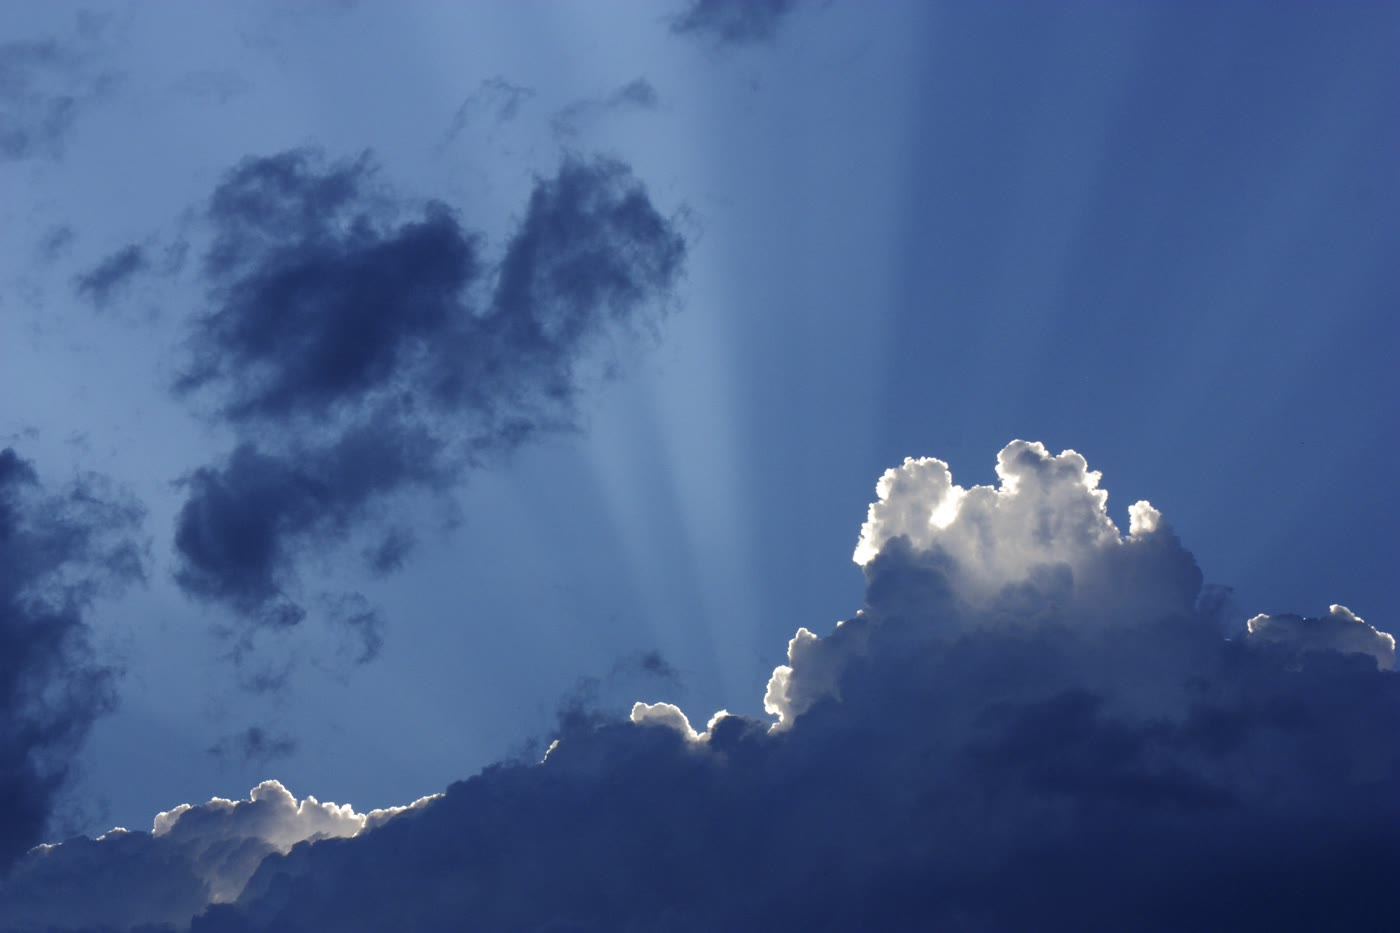
\includegraphics[width=0.55\linewidth]{images/book4/tyndall-sky.jpg}

{\small أشعة الشمس عبر فرجة في السحب: إنها مرئية لأن
\omterm{def:b3:colloids:colloid}{الهباء الجوي} في الهواء، من قطيرات وغبار، يشتت جزءًا من الضوء جانبيًا، وهذا
\omterm{def:b3:colloids:tyndall}{مفعول تندال} على مقياس السماء.}
\end{omfigure}

\section{استقرار الغروانيات}

يتجاذب جسيمان غروانيان دائمًا على مدى قصير بقوى فان دير
فالس. وفي الماء، تحمل معظم الجسيمات أيضًا شحنة (مجموعات سطحية
متأينة، وأيونات ممتزة)، تحيط بها \omterm{def:b3:electrode-kinetics:double-layer}{طبقة منتشرة} من الأيونات المضادة، أي الطبقة
المزدوجة في \cref{ch:b3:electrode-kinetics}. وحين يقترب جسيمان، تتداخل
طبقتاهما المنتشرتان وتتنافران.

\begin{definition}[جهد زيتا]\label{def:b3:colloids:zeta}
\emph{جهد زيتا}\index{جهد زيتا} $\zeta$ لجسيم هو الجهد
الكهربائي عند مستوي انزلاقه، وهو الحد داخل الطبقة المزدوجة بين
السائل الذي يتحرك مع الجسيم والسائل الذي لا يتحرك؛ ويُقاس
من سرعة الجسيمات في مجال كهربائي
(الرحلان الكهربائي).
\end{definition}

\begin{omfigure}
\begin{tikzpicture}[font=\scriptsize]
  \fill[black!20] (0,0) circle (1.2);
  \foreach \a in {0,30,...,330}{\node at (\a:1.05) {$-$};}
  \draw[omDef, dashed] (0,0) circle (1.55);
  \foreach \a in {15,45,...,345}{\draw[omDef, fill=omDef!15] (\a:1.38) circle (0.11); \node at (\a:1.38) {\tiny$+$};}
  \draw[omThm, thick, densely dotted] (0,0) circle (1.85);
  \foreach \a/\r/\s in {10/2.2/+, 50/2.5/+, 95/2.3/-, 130/2.7/+, 175/2.2/+, 215/2.6/-, 250/2.3/+, 290/2.8/+, 345/2.6/+}{
    \draw[black!60, fill=white] (\a:\r) circle (0.11); \node at (\a:\r) {\tiny$\s$};}
  \draw[->, black!60] (2.6,1.6) node[anchor=west] {\foreignlanguage{arabic}{طبقة شتيرن}} -- (40:1.6);
  \draw[->, omThm] (2.6,-1.4) node[anchor=west] {\foreignlanguage{arabic}{مستوي الانزلاق: $\zeta$}} -- (-30:1.87);
  \node at (0,0) {\foreignlanguage{arabic}{الجسيم}};
  \node[anchor=west] at (2.9,0.2) {\foreignlanguage{arabic}{الطبقة المنتشرة}};
\end{tikzpicture}

{\small جسيم مشحون سالبًا مع طبقته المزدوجة: طبقة شتيرن متراصة
من الأيونات المضادة، ومستوي الانزلاق خلفها مباشرة، حيث يُعرَّف \omterm{def:b3:colloids:zeta}{جهد
زيتا}، \omterm{def:b3:electrode-kinetics:double-layer}{والطبقة المنتشرة}، التي تفوق فيها الأيوناتُ المضادة
الأيوناتِ المرافقة عددًا على بضعة أطوال ديباي.}
\end{omfigure}

\begin{theorem}[نظرية DLVO]\label{thm:b3:colloids:dlvo}
من أجل كرتين نصف قطرهما $a$ تفصلهما فجوة $h \ll a$، وجهد طبقتهما المنتشرة
$\psi$ وثابت هاماكر $A$، تكون طاقة التآثر، عند الجهود المنخفضة،
\[
  V(h) = 2\pi\varepsilon_r\varepsilon_0a\psi^2\ln\bigl(1 + \eu^{-\kappa h}\bigr) - \frac{Aa}{12h} .
\]
الحد الأول، التنافر بين الطبقتين المزدوجتين، يتخامد على \omterm{def:b3:electrode-kinetics:double-layer}{طول ديباي} $\kappa^{-1}$؛
والثاني، تجاذب فان دير فالس، لا يتوقف على الملح. ولمجموعهما
حاجز طاقي عند بضعة أطوال ديباي حين يكون تركيز الملح
منخفضًا، ولا حاجز فوق تركيز حرج.
\end{theorem}

\begin{proof}[برهان جزئي]
نقبل الصيغتين كلتيهما (التنافر من تداخل طبقتي غوي--تشابمان
في تقريب ديرياغين، والتجاذب من جمع تآثرات لندن
على الجسمين). ورفع الشدة الأيونية يرفع $\kappa$
(\cref{prop:b3:electrode-kinetics:debye-length}): فيتلاشى التنافر عندئذ عند
قيم أصغر للفجوة $h$، حيث يكون التجاذب، الذي ينمو وفق $1/h$، أقوى؛ فتتناقص القيمة العظمى
للطاقة $V$ وتنعدم أخيرًا.
\end{proof}

\begin{omfigure}
\begin{tikzpicture}
\begin{axis}[width=0.72\linewidth, height=5.6cm, xmin=0, xmax=30, ymin=-40, ymax=45,
  axis lines=left, xlabel={\foreignlanguage{arabic}{الفجوة \babelsublr{$h$ / nm}}}, ylabel={$V/kT$},
  tick label style={font=\small}, label style={font=\small},
  legend style={font=\scriptsize, draw=none, at={(0.98,0.98)}, anchor=north east}, legend cell align=left]
\addplot[omDef, thick] table[x=h_nm, y=I1] {figdata/out/bachelor-3-dlvo.dat};
\addplot[black!60, thick] table[x=h_nm, y=I10] {figdata/out/bachelor-3-dlvo.dat};
\addplot[omThm, thick] table[x=h_nm, y=I50] {figdata/out/bachelor-3-dlvo.dat};
\addplot[black, thick, dashed] table[x=h_nm, y=I200] {figdata/out/bachelor-3-dlvo.dat};
\draw[black!30] (axis cs:0,0) -- (axis cs:30,0);
\legend{\qty{1}{mM}, \qty{10}{mM}, \qty{50}{mM}, \qty{200}{mM}}
\end{axis}
\end{tikzpicture}

{\small تآثر DLVO بين جسيمين نصف قطرهما \qty{100}{nm} (نموذج: جهد \omterm{def:b3:electrode-kinetics:double-layer}{الطبقة المنتشرة}
\qty{-30}{mV}، وثابت هاماكر \qty{2e-20}{J}) في ماء فيه ملح 1:1. عند \qty{1}{mM}
يُبقي حاجز قدره نحو $40\,kT$ الجسيمات متباعدة؛ وعند \qty{10}{mM} ينخفض إلى النصف؛
وقرب \qty{50}{mM} يختفي ويصير كل تصادم لاصقًا.}
\end{omfigure}

\begin{definition}[التخثر والتثبيت]\label{def:b3:colloids:stability}
\emph{التخثر}\index{تخثر} هو تجمّع الجسيمات الغروانية
بسبب فقدها تنافرها الكهروسكوني؛ و\emph{التندّف}\index{تندف}
تجمّع في ندف رخوة، تربط بينها غالبًا بوليمرات ممتزة. 
و\emph{تركيز التخثر الحرج}\index{تركيز التخثر الحرج}
(CCC) لإلكتروليت هو التركيز الذي يتخثر فوقه
\omterm{def:b3:colloids:colloid}{الغرواني} بسرعة. و\emph{التثبيت الفراغي}\index{تثبيت فراغي}
يُبقي الجسيمات متباعدة بسلاسل بوليمرية ممتزة أو مطعّمة،
يكلّف تداخلها إنتروبيا.
\end{definition}

\begin{proposition}[قاعدة شولتسه--هاردي]\label{prop:b3:colloids:schulze-hardy}
من أجل \omterm{def:b3:colloids:colloid}{غرواني} عالي الشحنة، يتغير \omterm{def:b3:colloids:stability}{تركيز التخثر الحرج}
لإلكتروليت كمقلوب القوة السادسة لشحنة $z$
أيوناته المضادة: $\text{CCC} \propto z^{-6}$، بالنسب $1 : \frac{1}{64} : \frac{1}{729}$ من أجل $z = 1, 2, 3$.
\end{proposition}

\begin{proof}[برهان جزئي]
لنعامل لوحين مستويين. عند جهد سطحي مرتفع يؤول تنافر الطبقتين المزدوجتين لكل
وحدة مساحة إلى $V_R = (64nkT/\kappa)\eu^{-\kappa h}$، حيث $n$ الكثافة العددية للإلكتروليت $z{:}z$،
مستقلًا عن الجهد (نقبله)؛ والتجاذب هو $V_A =
-A/(12\pi h^2)$. وعند التركيز الحرج يتلاشى الحاجز بالكاد: $V = 0$ و$\dd V/\dd h = 0$ عند
الفجوة نفسها. ولما كان $\dd V_R/\dd h = -\kappa V_R$ و$\dd V_A/\dd h = -2V_A/h$، فإن الشرطين يعطيان
$\kappa V_R = 2V_R/h$، ومنه $\kappa h = 2$، ثم $64nkT\eu^{-2}/\kappa = A\kappa^2/(48\pi)$، أي $n \propto \kappa^3$. ومع
$\kappa^2 = 2nz^2e^2/(\varepsilon kT)$، $\kappa^3 \propto (nz^2)^{3/2}$ و$n \propto n^{3/2}z^3$: ومنه $n \propto z^{-6}$.
\end{proof}

\begin{omfigure}
\begin{tikzpicture}[font=\small, >=Stealth]
  \foreach \x/\lab/\v in {0/\ce{Na+}/1, 2.6/\ce{Ca^{2+}}/{1/64}, 5.2/\ce{Al^{3+}}/{1/729}}{
    \node at (\x,0) {\lab};
    \node[font=\scriptsize] at (\x,-0.45) {CCC $\times\,\v$};}
  \draw[->, thick, omDef] (-0.8,-0.95) -- (6.0,-0.95) node[midway, below, font=\scriptsize] {\foreignlanguage{arabic}{جرعة أصغر لتخثير غرواني سالب}};
\end{tikzpicture}

{\small قاعدة شولتسه--هاردي \omterm{def:b3:colloids:colloid}{لغرواني} مشحون سالبًا: ينخفض \omterm{def:b3:colloids:stability}{تركيز التخثر
الحرج} كالقوة السادسة لشحنة الأيون المضاد.}
\end{omfigure}

تفسّر القاعدة لماذا تكون أملاح الألومنيوم فعالة إلى هذا الحد في ترويق الماء، 
ولماذا تُلقي الأنهار حمولتها من الطين حيث تلتقي بماء البحر المالح.

\begin{method}[اختيار جرعة المخثّر]\label{met:b3:colloids:coagulant-dose}
\begin{enumerate}
  \item قِس \omterm{def:b3:colloids:stability}{تركيز التخثر الحرج} لإلكتروليت مرجعي من أجل المعلَّق (اختبارات
        الجرار بجرعات متزايدة، مع مراقبة الترسب).
  \item انقله إلى الأيون المضاد للمخثّر بقاعدة شولتسه--هاردي.
  \item حوّله إلى كتلة ملح لكل متر مكعب باستعمال صيغته؛ وأضف ما يكفي
        للحلمأة وللقلوية التي يستهلكها.
  \item تجنّب الجرعة الزائدة: فالأيونات المضادة العالية الشحنة قد تعكس إشارة
        شحنة الجسيمات فتعيد تثبيتها.
\end{enumerate}
\end{method}

\section{الغروانيات في العمل}

\begin{definition}[التوازن بين المحب للماء والمحب للدهون]\label{def:b3:colloids:hlb}
\emph{التوازن بين المحب للماء والمحب للدهون}\index{توازن بين المحب للماء والمحب للدهون}
(HLB) \omterm{def:b3:colloids:surfactant}{لمادة فعالة سطحيًا غير أيونية} هو، في سلّم غريفين، $20$ مرة الكسر
الكتلي لجزئها المحب للماء: فالقيم المنخفضة (3 إلى 6) تلائم مستحلبات الماء في
الزيت، والقيم المرتفعة (8 إلى 18) مستحلبات الزيت في الماء والمنظفات.
\end{definition}

المستحلبات غير مستقرة ترموديناميكيًا، إذ تحمل كل قطيرة
طاقة بينية؛ وتجعلها المستحلِبات مستقرة حركيًا بخفض تلك
الطاقة وبإضافة طبقة منفِّرة، مشحونة أو فراغية، حول كل قطيرة.
والمايونيز \omterm{def:b3:colloids:colloid}{مستحلب} زيت في ماء فيه من الزيت الكثير (نحو أربعة أخماس
الحجم) حتى إن القطيرات تنضغط بعضها على بعض، وهذا ما يجعله
صلبًا لينًا. وتُثبَّت الرغاوى بمواد فعالة سطحيًا تبطّئ تصريف
الأغشية السائلة بين الفقاعات؛ أما مضادات \omterm{def:b3:colloids:colloid}{الرغوة}، وهي غالبًا زيوت السيليكون، فتنتشر على تلك
الأغشية وتكسرها. وفي محطات مياه الشرب، تخثّر أملاح الألومنيوم أو الحديد(III)
الطين والغروانيات العضوية التي تجعل ماء النهر عكرًا؛ 
ويجرف الهيدروكسيد الذي تكوّنه الندف إلى الأسفل في أثناء ترسبه. وتُبقى الجسيمات
النانوية الفلزية مشتتة بأيونات السترات الممتزة (كهروسكونيًا) أو بسلاسل بوليمرية
مرتبطة بالثيول (فراغيًا).

\begin{inthelab}[حلقة دو نوي]
تُعلَّق حلقة من البلاتين، تُنظَّف بتمريرها في اللهب، بميزان وتُغمر
أفقيًا في السائل، ثم تُرفع ببطء. وتمر القوة اللازمة لسحبها
عبر السطح بقيمة عظمى؛ وهذه القوة، مقسومةً على ضعف محيط
الحلقة ومصحَّحةً لشكل الهلالة المرفوعة، تعطي
\omterm{def:b3:colloids:surface-tension}{التوتر السطحي}. ويبدأ قياس سلسلة من محاليل \omterm{def:b3:colloids:surfactant}{مادة فعالة سطحيًا} من المحلول الأكثر
تمديدًا، مع شطف الحلقة بين العيّنات.
\end{inthelab}

\begin{safety}{\ghs[0.8cm]{GHS02}\ghs[0.8cm]{GHS05}\ghs[0.8cm]{GHS07}}
% ledger: ghs4:SDS, ghs4:Al2SO43
مسحوق دوديسيل كبريتات الصوديوم: صلب قابل للاشتعال، ضار إذا ابتُلع، يسبب
تلفًا شديدًا للعين، ويهيج المسالك التنفسية؛ يوزن دون إثارة
الغبار، مع حماية العينين. وكبريتات الألومنيوم (\ghs[0.6cm]{GHS05}): تسبب تلفًا شديدًا
للعين.
\end{safety}

\begin{history}[تندال والمجهر الفائق]
بيّن جون تندال في سنة 1869 أن حزمة ضوئية تصير مرئية في هواء محمّل
بجسيمات دقيقة وغير مرئية في هواء خالٍ منها، وأن الضوء المشتت
مائل إلى الزرقة ومستقطب. وبنى ريتشارد جيغموندي، الذي كان يدرس اللون الأحمر لصولات
الذهب، مع هنري زيدنتوبف في سنة 1903 المجهر الفائق، الذي يضيء
\omterm{def:b3:colloids:colloid}{الغرواني} من الجانب ويُظهر كل جسيم نقطةً من الضوء المشتت
على خلفية مظلمة، أصغر من أن يُميَّز لكنه قابل للعدّ. ونال
جائزة نوبل في الكيمياء لسنة 1925 عن أعماله في الغروانيات.
\end{history}

\section{تمارين}

\begin{exercise}[$\star$]\label{exo:b3:colloids:1}
% ledger: st:H2O.25C
احسب الضغط داخل فقاعة هواء قطرها \qty{1.0}{\micro m} في الماء عند
\qty{25}{\celsius} (في الخارج: \qty{1.0}{bar}).
\end{exercise}

\begin{exercise}[$\star$]\label{exo:b3:colloids:2}
% ledger: st:H2O.25C
احسب ضغط بخار قطيرة ماء نصف قطرها \qty{10}{nm} نسبةً إلى
الماء المستوي عند \qty{25}{\celsius} ($V_{\mathrm m} = \qty{18.07}{cm^3/mol}$).
\end{exercise}

\begin{exercise}[$\star$]\label{exo:b3:colloids:3}
سائل فيه $\gamma_{\mathrm{LV}} = \qty{72}{mN/m}$ على صلب فيه $\gamma_{\mathrm{SV}} = \qty{40}{mN/m}$ و$\gamma_{\mathrm{SL}} =
\qty{20}{mN/m}$ (معطيات التمرين): احسب \omterm{def:b3:colloids:wetting}{زاوية التماس}. هل \omterm{def:b3:colloids:wetting}{يبلّل} الصلب؟
\end{exercise}

\begin{exercise}[$\star$]\label{exo:b3:colloids:4}
% ledger: eps:H2O.25C
احسب \omterm{def:b3:electrode-kinetics:double-layer}{طول ديباي} في الماء عند \qty{25}{\celsius} من أجل \qty{0.010}{mol/L} من NaCl ومن
\ce{MgSO4}.
\end{exercise}

\begin{exercise}[$\star\star$]\label{exo:b3:colloids:5}
قبيل تركيزها المذيلي الحرج، ينخفض \omterm{def:b3:colloids:surface-tension}{التوتر السطحي} \omterm{def:b3:colloids:surfactant}{لمادة فعالة سطحيًا} أيونية (1:1، دون ملح)
بمقدار \qty{12.6}{mN/m} لكل وحدة من $\ln c$ عند \qty{25}{\celsius}. احسب الفائض السطحي 
والمساحة لكل جزيء.
\end{exercise}

\begin{exercise}[$\star\star$]\label{exo:b3:colloids:6}
التوترات السطحية \omterm{def:b3:colloids:surfactant}{لمادة فعالة سطحيًا غير أيونية}: 52.0 و45.5 و39.1 و33.4 و33.3 
و\qty{33.4}{mN/m} عند $\log c = -5.0$ و$-4.5$ و$-4.0$ و$-3.5$ و$-3.0$ و$-2.5$ (معطيات التمرين).
قدّر \omterm{def:b3:colloids:micelle}{التركيز المذيلي الحرج}.
\end{exercise}

\begin{exercise}[$\star\star$]\label{exo:b3:colloids:7}
من أجل دوديسيل كبريتات الصوديوم، خذ $v = \qty{0.350}{nm^3}$ و$l = \qty{1.67}{nm}$ و$a_0 = \qty{0.60}{nm^2}$؛ ومن أجل
ليبيد له سلسلتان من هذا النوع، $2v$ و$l$ نفسه و$a_0 = \qty{0.65}{nm^2}$ (معطيات
التمرين). تنبّأ بشكل تجمعاتهما.
\end{exercise}

\begin{exercise}[$\star\star$]\label{exo:b3:colloids:8}
يتخثر \omterm{def:b3:colloids:colloid}{صول} مشحون سالبًا عند \qty{60}{mM} من NaCl. تنبّأ \omterm{def:b3:colloids:stability}{بتركيز التخثر الحرج} مع \ce{CaCl2}
ومع \ce{AlCl3}. وماذا يفعل \ce{Na3PO4}؟
\end{exercise}

\begin{exercise}[$\star\star$]\label{exo:b3:colloids:9}
% ledger: cmc:C12E6
احسب قيمة HLB وفق غريفين لإيثر أحادي الدوديسيل لسداسي إيثيلين الغليكول،
\ce{C12H25(OCH2CH2)6OH}، الذي جزؤه المحب للماء $\ce{(OCH2CH2)6OH}$. هل يلائم
\omterm{def:b3:colloids:colloid}{مستحلب} زيت في ماء؟
\end{exercise}

\begin{exercise}[$\star\star\star$]\label{exo:b3:colloids:10}
يحتوي مُشتَّت على قطيرات نصف قطرها 50 و\qty{500}{nm}. باستعمال \omterm{thm:b3:colloids:kelvin}{معادلة كلفن}
مطبَّقةً على الذوبانية، فسّر أيها ينمو وأيها يصغر، ولماذا
تخشُن المستحلبات مع الزمن حتى دون اندماج.
\end{exercise}

\begin{exercise}[$\star\star\star$]\label{exo:b3:colloids:11}
بيّن انطلاقًا من ضغط لابلاس أن السائل يرتفع إلى الارتفاع $h = 2\gamma\cos\theta/(\rho gr)$ في
أنبوب شعري نصف قطره $r$، واحسبه للماء ($\theta = 0$، نصف قطر \qty{0.10}{mm}).
\end{exercise}

\begin{exercise}[$\star\star\star$]\label{exo:b3:colloids:12}
باستعمال شكل DLVO، فسّر لماذا تؤدي إضافة \qty{100}{mM} من NaCl إلى \omterm{def:b3:colloids:colloid}{صول} مستقر عند \qty{1}{mM}
إلى تخثره، بينما لا تغيّر إضافة بوليمر غير ممتز
الحاجز، أما البوليمر المطعَّم على الجسيمات فيستطيع إبقاءها متباعدة مهما كان تركيز
الملح.
\end{exercise}

% keep the heading with its problem box, which fills a page by itself
\clearpage
\enlargethispage{3\baselineskip}
\section{مسألة: ترويق الماء الموحل بالشبّ}

\begin{problem}[{مسألة نهاية الأسبوع --- ترويق الماء الموحل بالشبّ:
الطبقة المزدوجة لجسيمات الطين، وحاجز DLVO، وقاعدة شولتسه--هاردي، 
وجرعة كبريتات الألومنيوم}]
\label{pb:b3:colloids:1}
% ledger: eps:H2O.25C, visc:H2O.25C
تستقبل محطة لمعالجة المياه ماءً يسرًا عكرًا: جسيمات طين نصف قطرها
\qty{100}{nm} وكثافتها \qty{2650}{kg/m^3}، وجهد \omterm{def:b3:electrode-kinetics:double-layer}{طبقتها المنتشرة} \qty{-30}{mV}، في
ماء يحوي \qty{1.0}{mM} من \ce{NaHCO3}. وتبيّن اختبارات الجرار أن الجسيمات تتخثر
بسرعة فوق \qty{50}{mM} من NaCl (معطيات المسألة). وتعالج المحطة \qty{1000}{m^3} في
الساعة بكبريتات الألومنيوم، $\ce{Al2(SO4)3}$ ($M = \qty{342.3}{g/mol}$).

\medskip\noindent\textbf{الجزء الأول --- \omterm{def:b3:colloids:colloid}{غرواني} مستقر.}
\begin{enumerate}
  \item لماذا تحمل جسيمات الطين في الماء شحنة سالبة؟
  \item احسب الشدة الأيونية للماء.
  \item احسب \omterm{def:b3:electrode-kinetics:double-layer}{طول ديباي} فيه.
  \item قارنه بنصف قطر الجسيم. أي تقريب لصيغة DLVO
        يسوّغه ذلك؟
  \item احسب سرعة ترسب جسيم بقانون ستوكس، $v =
        2\Delta\rho\,gr^2/9\eta$ ($\eta = \qty{0.89}{mPa.s}$)، بالمليمتر في اليوم.
  \item لماذا لا تلتصق الجسيمات بعضها ببعض حين تتصادم؟
\end{enumerate}

\medskip\noindent\textbf{الجزء الثاني --- حاجز DLVO.}
\begin{enumerate}[resume]
  \item اكتب طاقة DLVO لجسيمين.
  \item اقرأ على الشكل الحاجز عند \qty{1}{mM}، بوحدة $kT$.
  \item كم مرة يعبر جسيمان متصادمان حاجزًا كهذا؟
  \item ماذا يحدث للحاجز قرب \qty{50}{mM}؟
  \item فسّر لماذا تخفض إضافة الملح الحاجز.
\end{enumerate}

\medskip\noindent\textbf{الجزء الثالث --- شولتسه--هاردي.}
\begin{enumerate}[resume]
  \item اذكر القاعدة.
  \item تنبّأ \omterm{def:b3:colloids:stability}{بتركيز التخثر الحرج} للأيون \ce{Ca^{2+}}.
  \item تنبّأ \omterm{def:b3:colloids:stability}{بتركيز التخثر الحرج} للأيون \ce{Al^{3+}}.
  \item لماذا لا تهم إلا كاتيونات المخثّر في هذا \omterm{def:b3:colloids:colloid}{الغرواني}؟
  \item لماذا لا يكاد يكون لكبريتات الشبّ دور في \omterm{def:b3:colloids:stability}{التخثر}؟
\end{enumerate}

\medskip\noindent\textbf{الجزء الرابع --- الجرعة.}
\begin{enumerate}[resume]
  \item احسب كمية \ce{Al^{3+}} اللازمة لكل متر مكعب.
  \item استنتج كمية $\ce{Al2(SO4)3}$ لكل متر مكعب.
  \item استنتج كتلتها لكل متر مكعب.
  \item استنتج الكتلة التي تستعملها المحطة في الساعة.
  \item في الماء، يتحلمأ \ce{Al^{3+}} ويتفاعل مع الهيدروجين كربونات. اكتب
        المعادلة الموزونة التي يتكوّن فيها \ce{Al(OH)3}.
  \item ما نسبة الهيدروجين كربونات التي تستهلكها الجرعة؟ وهل يتغير
        pH كثيرًا؟
  \item لماذا قد تعيد الجرعة الزائدة الماء عكرًا؟
  \item اذكر النتيجة: الكتلة الدنيا من كبريتات الألومنيوم لكل متر مكعب.
\end{enumerate}
\end{problem}
